\runningheader{Oppgave k), frivillig }{}{Side \thepage\ av \numpages}


% ********************************************************
% oppgave k) 
% ********************************************************  
\item[k)]
  Kopier modellen fra j), og erstatt {\sf  Constant}-blokken
  med en {\sf  Ramp}-blokk og bygg modellen om som vist under.

  \begin{figure}[H]
    \centering
    \hspace*{0mm}\scalebox{0.8}{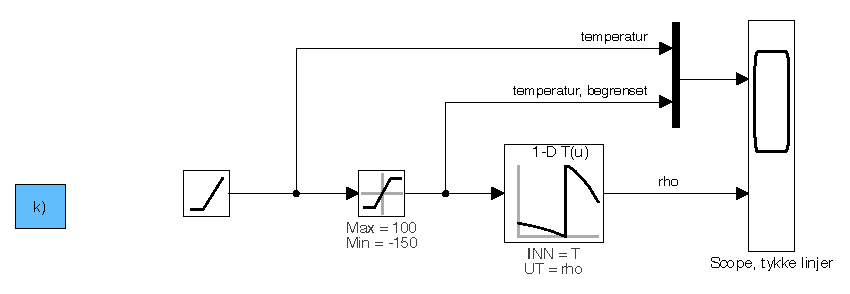
\includegraphics{2k.pdf}}
  \end{figure}

  Spesifiser rampen på en slik måte at
  temperaturen stiger fra $-200^{\circ}$C til $+200^{\circ}$C i løpet av
  simuleringstiden på 25 sekund ut fra følgende sammenheng
    \begin{equation}
    \label{eq:F_tb}
    T(t) = -200 + a{\cdot}t 
  \end{equation}
  {\color{red}La simuleringstiden fortsatt være 25 sekund.  }

      {\bf Svar på følgende spørsmål:    }

\begin{enumerate}[label=k\arabic*)]
        \item Hva blir verdien av $a$?
  \item   Simuler modellen og ta med resultatet i
    innleveringen din.    Forklar hva som skjer i simuleringen.

\item Ved hvilket tidspunktet er temperaturen $T{=}-20^{\circ}$C? Er
  avlest tetthet den samme som i oppgave i)?  
    
\item   Forstørr området mellom $12{<}t{<}17$ sekund på samme måte som
   vist med blå kurve i figur~\ref{fig:akima}.  Få frem at 
  kurven for tettheten består av lineære elementer som viser den lineære
  interpolasjonen som blokken utfører.

  \end{enumerate}
  
